\chapter{Python}
\begin{center}
    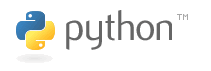
\includegraphics[width=140px]{img/python.png} \\
    \textbf{\href{http://python.org}{www.python.org}}
\end{center}
\begin{quote}
    \textit{Python is a programming language that lets you work more quickly and integrate your systems more effectively. You can learn to use Python and see almost immediate gains in productivity and lower maintenance costs.}
\end{quote}

\section{IPython}
Python selbst kommt mit einer interaktiven Kommandozeile (genauer: eine REPL\footnote{ read–eval–print loop}-Umgebung). Um einen Einblick in die Sprache zu erhalten, ist diese eigentlich vollkommen ausreichend. Sie bietet die Möglichkeit, interaktiv mit der Sprache in Kontakt zu kommen. IPython erlaubt zusätzlich, auf die Shell zuzugreifen und interaktive Sitzungen zu speichern.
Gestartet wird IPython auf der Kommandozeile mit
\begin{verbatim}
$ ipython
\end{verbatim}
und meldet sich (zum Beispiel hier unter OS X mit Python 3.2.3) mit der Ausgabe
\begin{verbatim}
Python 3.2.3 (default, Apr 13 2012, 00:15:25) 
Type "copyright", "credits" or "license" for more information.

IPython 0.13 -- An enhanced Interactive Python.
?         -> Introduction and overview of IPython's features.
%quickref -> Quick reference.
help      -> Python's own help system.
object?   -> Details about 'object', use 'object??' for extra details.

In [1]: 
\end{verbatim}
Um IPython zu beenden gibt es die Befehle \texttt{exit}, \texttt{exit()}, \texttt{quit}, \texttt{quit()} und natürlich Ctrl-D.

\section{Syntax}
Grundsätzlich ist die Python-Syntax sehr einfach und intuitiv. In vielen Punkten erinnert sie eher an eine Scriptsprache. In einer interaktiven Sitzung (z.B. IPython) können zum Einstieg einfache mathematische Berechnungen durchgeführt werden:
\begin{verbatim}
In [1]: 1+2
Out[1]: 3

In [2]: 1-2
Out[2]: -1

In [3]: 1*2
Out[3]: 2

In [4]: 1/2
Out[4]: 0.5
\end{verbatim}

\subsection{Operatoren}
Wie aus dem obigen Beispiel hervorgeht, gibt es die mathematischen Operatoren \texttt{+},\texttt{-},\texttt{*} und \texttt{/}. Die folgenden Tabellen geben einen Überblick über die weiteren Operatoren.

\subsection{Variablen}

\section{Bibliotheken}
\subsection{Numpy}
\subsection{Scipy}
\subsection{Matplotlib}

\section{Weiterführende Links}
\begin{itemize}
  \item Learn Python The Hard Way (Python 2): \url{http://learnpythonthehardway.org/}
  \item Dive Into Python 3: \url{http://www.diveintopython3.net/}
  \item Python v3 documentation: \url{http://docs.python.org/py3k/}
  \item Tentative NumPy Tutorial: \url{http://www.scipy.org/Tentative\_NumPy\_Tutorial}
  \item Numpy and Scipy Documentation: \url{http://docs.scipy.org/doc/}
  \item Matplotlib Documentation: \url{http://matplotlib.org/1.2.0/contents.html}
  \item Matplotlib Gallery: \url{http://matplotlib.org/1.2.0/gallery.html}
  \item Python Uncertainties package: \url{http://packages.python.org/uncertainties/}
\end{itemize}
